% This file is based on the header.tex file from https://github.com/pep-dortmund/toolbox-workshop-protocol-template
% The original file is licensed under the GPL-3.0 license
\documentclass[
  bibliography=totoc,     % Literatur im Inhaltsverzeichnis
  captions=tableheading,  % Tabellenüberschriften
  titlepage=firstiscover, % Titelseite ist Deckblatt
]{scrartcl}

% Paket float verbessern
\usepackage{scrhack}

% Warnung, falls nochmal kompiliert werden muss
\usepackage[aux]{rerunfilecheck}

% unverzichtbare Mathe-Befehle
\usepackage{amsmath}
% viele Mathe-Symbole
\usepackage{amssymb}
% Erweiterungen für amsmath
\usepackage{mathtools}

% Fonteinstellungen
\usepackage[T1]{fontenc}
\usepackage{lmodern}

% Wenn man andere Schriftarten gesetzt hat,
% sollte man das Seiten-Layout neu berechnen lassen
\recalctypearea{}

% deutsche Spracheinstellungen
% change to \usepackage[english]{babel} if you are writing in English
\usepackage[ngerman]{babel}

% Zahlen und Einheiten
\usepackage[
  locale=DE,                   % deutsche Einstellungen
  separate-uncertainty=true,   % immer Unsicherheit mit \pm
  per-mode=symbol-or-fraction, % / in inline math, fraction in display math
]{siunitx}

% chemische Formeln
\usepackage[
  version=4,
  math-greek=default, % ┐ mit unicode-math zusammenarbeiten
  text-greek=default, % ┘
]{mhchem}

% richtige Anführungszeichen
\usepackage[autostyle]{csquotes}

% schöne Brüche im Text
\usepackage{xfrac}

% Standardplatzierung für Floats einstellen
\usepackage{float}
\floatplacement{figure}{htbp}
\floatplacement{table}{htbp}

% Floats innerhalb einer Section halten
\usepackage[
  section, % Floats innerhalb der Section halten
  below,   % unterhalb der Section aber auf der selben Seite ist ok
]{placeins}

% Seite drehen für breite Tabellen: landscape Umgebung
\usepackage{pdflscape}

% Captions schöner machen.
\usepackage[
  labelfont=bf,        % Tabelle x: Abbildung y: ist jetzt fett
  font=small,          % Schrift etwas kleiner als Dokument
  width=0.9\textwidth, % maximale Breite einer Caption schmaler
]{caption}
% subfigure, subtable, subref
\usepackage{subcaption}

% Grafiken können eingebunden werden
\usepackage{graphicx}

% schöne Tabellen
\usepackage{tabularray}
\UseTblrLibrary{booktabs, siunitx}

% Verbesserungen am Schriftbild
\usepackage{microtype}

% Literaturverzeichnis
\usepackage[
  backend=biber,
]{biblatex}
% Quellendatenbank
\addbibresource{lit.bib}

% Hyperlinks im Dokument
\usepackage[
  german,
  unicode,        % Unicode in PDF-Attributen erlauben
  pdfusetitle,    % Titel, Autoren und Datum als PDF-Attribute
  pdfcreator={},  % ┐ PDF-Attribute säubern
  pdfproducer={}, % ┘
]{hyperref}
% erweiterte Bookmarks im PDF
\usepackage{bookmark}

% Trennung von Wörtern mit Strichen
\usepackage[shortcuts]{extdash}


\author{%
  AUTOR A\\%
  \href{mailto:authorA@uni-kassel.de}{authorA@uni-kassel.de}\\%
  MatrNr.: 123456789\\%
  \and%
  AUTOR B\\%
  \href{mailto:authorB@uni-kassel.de}{authorB@uni-kassel.de}\\%
  MatrNr.: 234567890\\%
  \and%
  AUTOR C\\%
  \href{mailto:authorC@uni-kassel.de}{authorC@uni-kassel.de}\\%
  MatrNr.: 345678901\\%
}
\publishers{Betreuer: Arne Vereijken / Adrian Krone\\Universität Kassel – Institut für Physik und CINSaT}

\subject{V0}
\title{Beispielversuch: "Torsionsmodul"}
\date{%
  Durchführung: Datum
  \hspace{3em}
  Abgabe: Datum
}

\begin{document}

\maketitle
\thispagestyle{empty}
\tableofcontents
\newpage

\section{Theorie}
\label{sec:Theorie}
\section{Messprotokoll}
\textsl{In diesem Teil wird das Messprotokoll aus dem Original in ein ordentliches Format gebracht\footnote{Scan / Foto des Original Messprotokolls vom Versuchstag im Anhang}.}

\begin{figure}
    \centering
    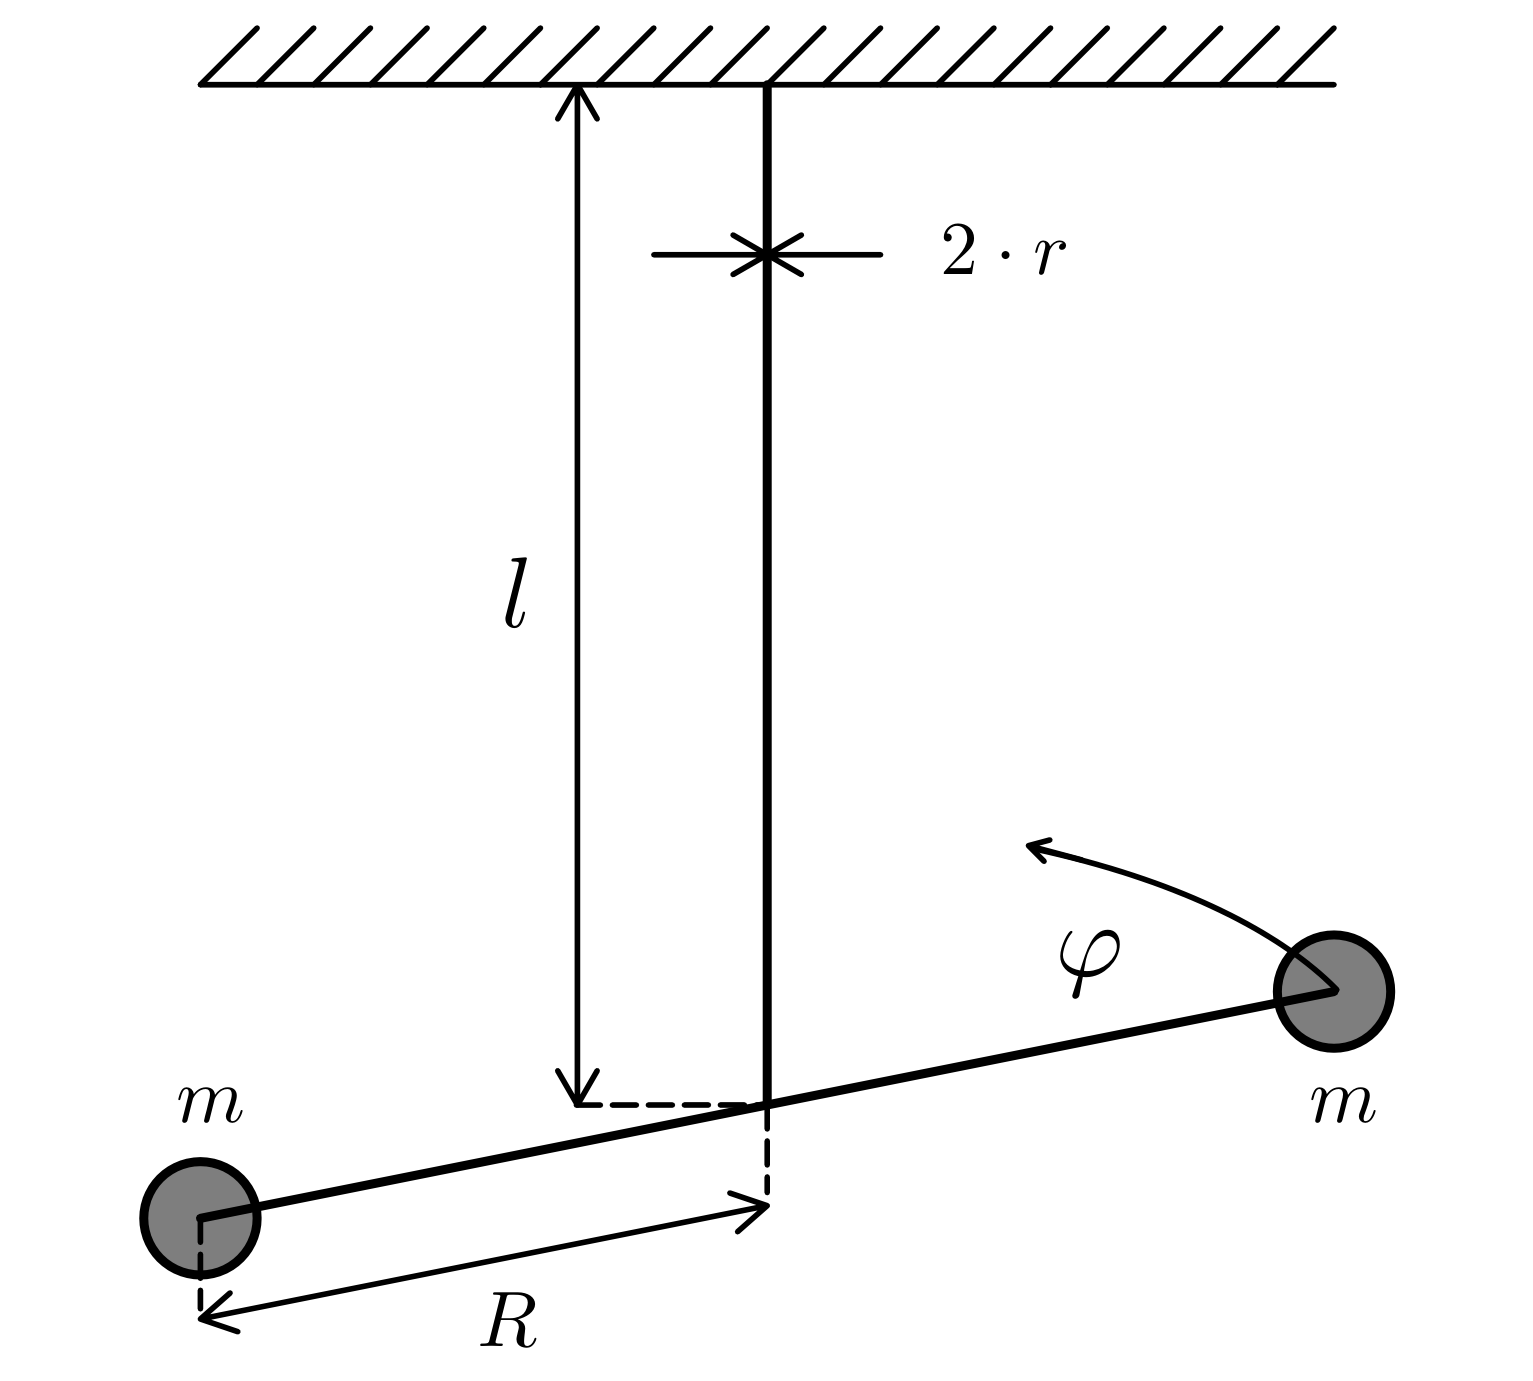
\includegraphics[width=0.6\textwidth]{plots/skizze.png}
    \caption{Skizze des Torsionspendels. \textsl{Zeichnen Sie hier eine sinvolle Skizze des Versuchsaufbaus und beschriften Sie diese inklusive aller Messpositionen und Konstanten.}}
    \label{fig:skizze}
\end{figure}

\subsection{Versuchsdurchführung}
Zuerst wurden die Abmessungen des Pendels sowie die für die Auswertung erforderlichen anderen Größen bestimmt (siehe Abb. \ref{fig:skizze}).
Außerdem wurden die Fehler für die einzelnen Messungen abgeschätzt.
Die Massen, die während der Versuchsdurchführung am Pendel angebracht wurden, wurden mit einer elektronischen Waage des Typs "`Kern CB12K1N"' gewogen.
Die Zeitmessung erfolgte mit einer elektronischen Stoppuhr des Typs "`Triple Timer"'.
Die Abmessungen des Pendels wurden mit einem Bandmaß bestimmt; für die Bestimmung des Durchmessers des Drahtes wurde eine Mikrometerschraube verwendet, deren Bezeichnung auf Grund von häufiger Benutzung nicht mehr erkennbar war. 

Bei der Durchführung wurde wie folgt vorgegangen: Zuerst wurde die Ruhelage des Pendels bestimmt. Von dort aus wurde dem Pendel eine Anfangsamplitude von einer Umdrehung gegeben.
Bei Starten des Pendels aus dieser Postion erfuhr es leichte vertikale Schwingungen um die horizontale Achse, welche über die Dauern der einzelnen Messungen bestehen blieben.
Die Zeitmessung erfolgte an demjenigen Umkehrpunkt der Pendelbewegung, bei dem die Pendelbewegung startete.

Der Messzeitraum am Pendel umfasste 30 Schwingungen bei der Massepositionierung am äußeren Rand des Pendels.
Bei den anderen Messungen wurde nur über einen Zeitraum von 25 Schwingungen gemessen, wobei versehentlich jeweils eine Schwingung zusätzlich gezählt und somit 26 Schwingungen aufgenommen wurden. Die Reduzierung der Schwingungsanzahl erfolgte aus Zeitgründen.
Aus demselben Grund wurden pro Positionierung der Massen nur zwei statt drei Messungen durchgeführt.

Während jeder Messung der Schwingungsdauern war zu beobachten, dass die Amplitude der Pendelbewegung über den Messzeitraum kontinuierlich abgenommen hat, sodass sie zum Ende einer jeden Messung um ca. 180$^\circ$ reduziert war.
Dies entspricht ca. 50\% der Startamplitude.

\subsection{Messwerte}
\textsl{Erstellen Sie hier eine Tabelle mit den Messwerten und den zugehörigen abgeschätzten Messfehlern.}

\begin{table}[ht]
    \centering
    \begin{tblr}{
        colspec=cc, rowsep=2pt,
        vlines{}, hline{1,2,3},    
        }
        Länge $l \;/\; \si{\meter}$ & Durchmesser $d \;/\; \si{\meter}$ \\
        \num{1,500(3)} & \num{5,0(2)e-4} \\
    \end{tblr}
    \caption{Gemessene Eigenschaften des Drahtes.}
    \label{tab:draht}
\end{table}
\begin{table}[ht]
    \centering
    \begin{tblr}{
        colspec=ccccc, rowsep=2pt,
        vlines{}, hline{1,2,4,8},
        cell{2}{2}={r=2}{c},
        cell{4}{2}={r=4}{c},
        cell{2}{3}={r=2}{c},
        cell{4}{3}={r=2}{c},
        cell{6}{3}={r=2}{c},
        }
        Messung & Masse $m \;/\; \si{\kilogram}$ & Position $R\;/\;\si{\meter}$ & $t \;/\; \si{\second}$ & \#Perioden n \\
        $t_{01}$ & -              &   -            & \num{755,53(100)} & 26 \\
        $t_{02}$ &                &                & \num{726,29(100)} & 25 \\
        $t_{11}$ & \num{0,393(1)} & \num{0,045(3)} & \num{806,59(100)} & 26 \\
        $t_{12}$ &                &                & \num{775,66(100)} & 25 \\
        $t_{21}$ &                & \num{0,200(3)} & \num{1637,8(10)}  & 30 \\
        $t_{22}$ &                &                & \num{1638,0(10)}  & 30 \\
    \end{tblr}
    \caption{Gemessene Zeiten der sechs Einzelmessungen.}
    \label{tab:messwerte}
\end{table}

\section{Auswertung}

Die Schwingungsdauern 
\begin{equation}
    T_i = \frac{1}{2}\left(\frac{t_{i1}}{n_{i1}} + \frac{t_{i2}}{n_{i2}}\right)
\end{equation}
ergeben sich aus den Messgrößen $t_{i1}$ und $t_{i2}$ der beiden Einzelmessungen über alle Perioden, jeweils dividiert durch die Zahl der Schwingungen pro Messung mit der jeweiligen Unsicherheit
\begin{equation}
    \sigma_{T_i} = \sqrt{\frac{\sigma_{t_{i1}}^2}{4 n_{i1}^2} + \frac{\sigma_{t_{i2}}^2}{4 n_{i2}^2}} ,
\end{equation}
welche nach dem Gaußschen Fehlerfortpflanzungsgesetz bestimmt wird.
Durch Einsetzen der gemessenen Werte aus Tabelle \ref{tab:messwerte} ergibt sich
\begin{align*}
    T_0 &= \qty{29,06(3)}{\second} \\
    T_1 &= \qty{31,02(3)}{\second} \\
    T_2 &= \qty{54,60(3)}{\second} .
\end{align*}
Die Federkonstante lässt sich nach Gleichung \eqref{eq:federkonstante} bestimmen
\begin{equation*}
    D = \qty{2,92(10)e-4}{\newton\meter}
\end{equation*}
mit der Unsicherheit\footnote{Dies ist erneut die Gaußsche Fehlerfortpflanzung. Diese muss nicht so ausführlich hingeschrieben werden wie hier.}
\begin{equation*}
    \sigma_D = \sqrt{\left(\frac{\partial D}{\partial m}\cdot \sigma_{m}\right)^2+\left(\frac{\partial D}{\partial R_1}\cdot \sigma_{R_1}\right)^2+\left(\frac{\partial D}{\partial R_2}\cdot \sigma_{R_2}\right)^2+\left(\frac{\partial D}{\partial T_1}\cdot \sigma_{T_1}\right)^2+\left(\frac{\partial D}{\partial T_2}\cdot \sigma_{T_2}\right)^2}
\end{equation*}
und den jeweiligen Ableitungen
\begin{align*}
    \frac{\partial D}{\partial m} &= 4\cdot \pi^2\cdot \frac{R_2^2 - R_1^2}{T_2^2 - T_1^2} \\
    \frac{\partial D}{\partial R_1} &= 4\cdot \pi^2\cdot m\cdot \frac{(-2)\cdot R_1}{T_2^2 - T_1^2} \\
    \frac{\partial D}{\partial R_2} &= 4\cdot \pi^2\cdot m\cdot \frac{2\cdot R_2}{T_2^2 - 
    T_1^2} \\
    \frac{\partial D}{\partial T_1} &= -4\cdot \pi^2\cdot m\cdot \frac{R_2^2 - R_1^2}{(T_2^2-T_1^2)^2}\cdot (-2)\cdot T_1 \\
    \frac{\partial D}{\partial T_2} &= -4\cdot \pi^2\cdot m\cdot \frac{R_2^2 - R_1^2}{(T_2^2 - T_1^2)^2}\cdot 2\cdot T_2 .
\end{align*}
Damit ist es möglich das Torsionsmodul des Stahldrahtes bzw. die Verdrillung nach Gleichung \eqref{eq:torsionsmodul} zu ermitteln:
\begin{equation*}
    G = \qty{7,1(12)e10}{\newton\per\square\meter}
\end{equation*}
Dabei wird die Unsicherheit mit
\begin{equation*}
    \sigma_G = \frac{2}{\pi} \sqrt{\left(\frac{l}{r^4} \cdot \sigma_D\right)^2 + \left(\frac{D}{r^4} \cdot \sigma_l\right)^2 + \left(\frac{4 \cdot D \cdot l}{r^5} \cdot \sigma_r\right)^2}
\end{equation*}
fortgepflanzt.
Mit der Messung ohne zusätzliche Massen $T_0$, der Gleichung \eqref{eq:schwingungsdauer} und der Gaußschen Fehlerfortpflanzung
\begin{equation*}
    \sigma_J = \sqrt{\left(\frac{T_0^2}{4 \pi^2} \cdot \sigma_D\right)^2 + \left(\frac{2 \cdot T_0 \cdot D}{4 \pi^2} \cdot \sigma_{T_0}\right)^2}
\end{equation*}
wird das Trägheitsmoment des Pendels bestimmt:
\begin{equation*}
    J = \qty{6,24(21)e-3}{\kilo\gram\meter\squared}
\end{equation*}

\section{Zusammenfassung und Diskussion}
Aus den durchgeführten Messungen haben sich die folgenden Größen für das Torsionspendel ergeben:
\begin{equation*}
    D = \qty{2,92(10)e-4}{\newton\meter}
\end{equation*}
\begin{equation*}
    G = \qty{7.1(12)e10}{\newton\per\square\meter}
\end{equation*}
\begin{equation*}
    J = \qty{6,24(21)e-3}{\kilo\gram\meter\squared}
\end{equation*}
Einen Vergleichswert aus der Literaur gibt es auf Grund des spezifischen Aufbaus des Experiments nur für das Torsionsmodul des Stahls. So findet sich in \cite{Walcher2004}: "`$\alpha$-Eisen: $G = \qty{0,84e4}{kp\per\milli\meter\squared}$"'. Dies entspricht einem Wert von $G = \qty{7.46e10}{\newton\per\square\meter}$, was innerhalb einer Standardabweichung des aus den Messungen bestimmten Wertes liegt.

Die relativ hohe Fehlertoleranz des experimentell bestimmten Torsionsmoduls ist in der Hauptsache durch die Genauigkeit der Messung des Drahtdurchmessers verursacht.
Für eine präzisere Bestimmung des Torsionsmoduls mit dem verwendeten Pendel, müsste der Durchmesser mit einer genaueren Mikrometerschraube gemessen werden.


\printbibliography{}

\end{document}